


\subsection{1.30 Гидридные комплексы переходных металлов. Способы получения и условия стабильности, геометрия, электронное строение, свойства.}
Водородные лиганды у переходных металлов традиционно и практически исключительно называют "гидридами" независимо от того, проявляются в их поведении гидридные свойства или нет (как мы увидим в дальнейшем, многие из этих "гидридов" являются довольно сильными кислотами). \\
Гидриды могут либо быть лигандами у одного атома металла (терминальные гидриды), либо служить мостиками между двумя или тремя атомами металла, либо занимать положение внутри клетки из атомов металла.  \\
Как правило, гидридные лиганды занимают обычные координационные места, т.е. они являются "стереохимически активными". \\
В качестве доказательства наиболее часто ссылаются на структуру $HMn(CO)_5$, длина связи $H-Mn$ составляет $1,60$ ангстрем, что равно сумме ковалентных радиусов $H$ и $M(I)$. \\
Связь $M-H$ прочнее $M-C$, первая лежит в пределах $190-250$ кДж/моль, а вторая -- $150-180 $ кДж/моль  	
\begin{figure} [H]
	\centering {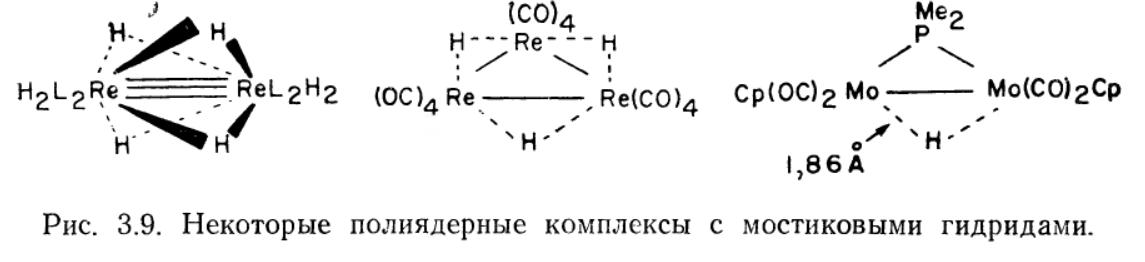
\includegraphics[scale=0.7]{oo2}}
\end{figure}
Система $M(\mu H)M$ всегда нелинейна, т.е. водород никогда не лежит на линии связи $M - M$. Такая геометрия обусловлена замкнутой трехцентровой двухэлектронной связью, поэтому расстояние $M - M$ в таких системах больше, чем в простой двухцентровой двухэлектронной связи металл-металл.
\begin{figure} [H]
	\centering {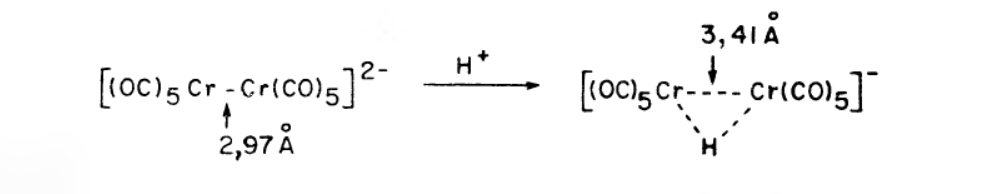
\includegraphics[scale=0.7]{oo3}}
\end{figure}
\textbf{Синтез}
\begin{itemize}
	\item Реакция окислительного присоединения $H_2$ к координационно ненасыщенным комплексам
	\begin{figure} [H]
		\centering {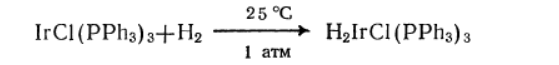
\includegraphics[scale=0.7]{oo4}}
	\end{figure}
	\item Реакция окислительного присоединения $H_2$ к координационно насыщенным комплексам
	\begin{figure} [H]
		\centering {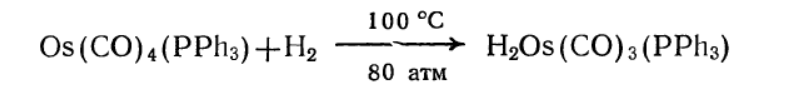
\includegraphics[scale=0.7]{oo5}}
	\end{figure}	
	\item Восстановлением в токе водорода
	\begin{figure} [H]
		\centering {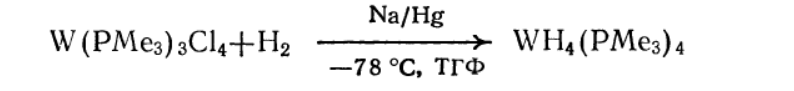
\includegraphics[scale=0.7]{oo6}}
	\end{figure}
	\item (некоторые) Гетеролиз $H_2$
	\begin{figure} [H]
		\centering {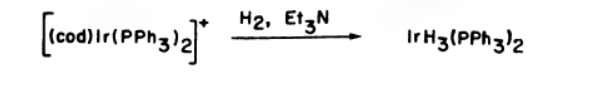
\includegraphics[scale=0.7]{oo7}}
	\end{figure}
	\item Гидрогенолиз связи металл-алкил
	\begin{figure} [H]
		\centering {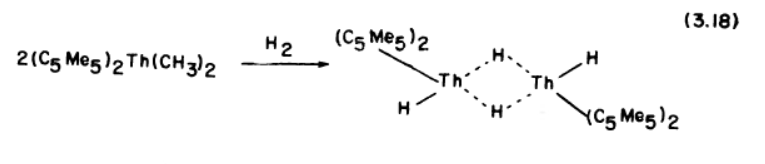
\includegraphics[scale=0.7]{oo8}}
	\end{figure}
	\item Гидрогенолиз одинарных связей металл-металл
	\begin{figure} [H]
		\centering {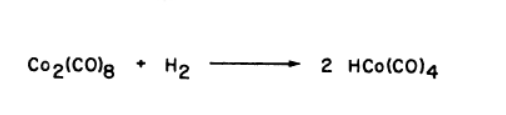
\includegraphics[scale=0.7]{oo9}}
	\end{figure}
	\item Гидрогенолиз двойных связей металл-металл
	\begin{figure} [H]
		\centering {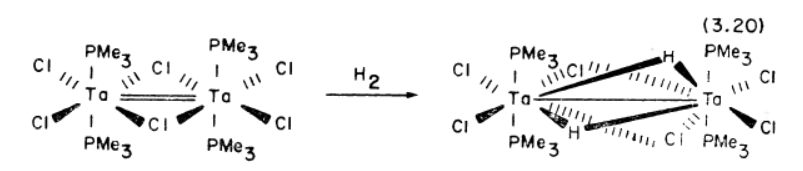
\includegraphics[scale=0.7]{oo10}}
	\end{figure}
\end{itemize}
\textbf{Кислотность гидридов:} \\
$HCo(CO)_4$ - намного более слабая кислота, чем хлорная, несколько более слабая, чем $HBr$ и $H_2SO_4$, и примерно такойже силы, как $HCl$ и  $HNO_3$. $H_2Fe(CO)_4$ имеет $pK_a - 4,0$ по первой ступени.
\begin{figure} [H]
	\centering {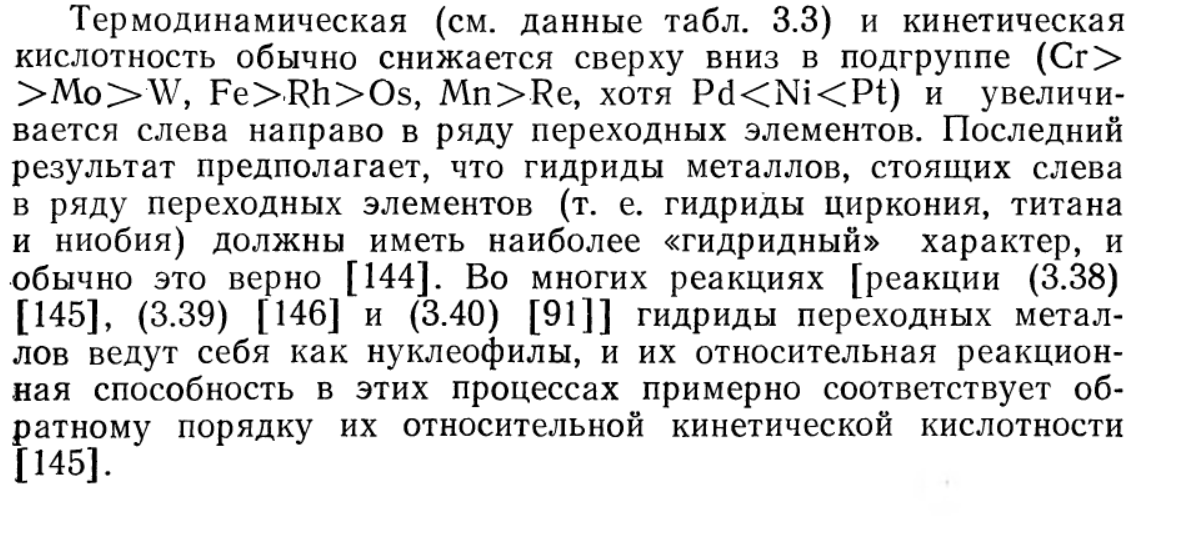
\includegraphics[scale=0.7]{oo11}}
\end{figure}
\begin{figure} [H]
	\centering {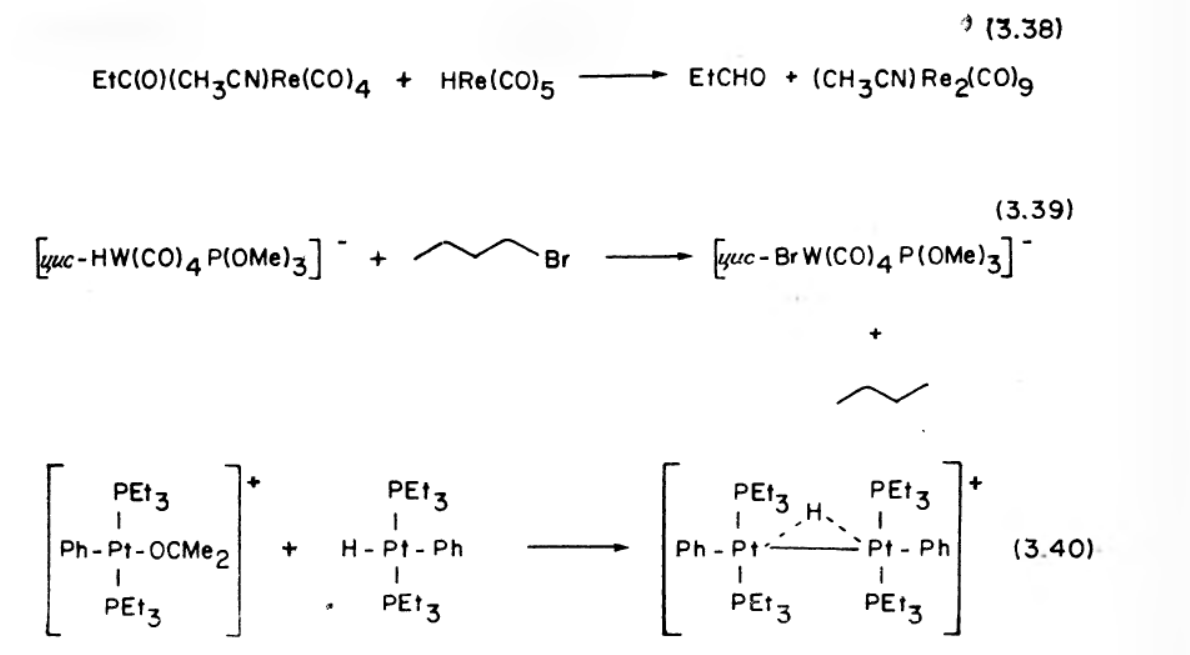
\includegraphics[scale=0.7]{oo12}}
\end{figure}
\textbf{Cвойства:} 
\begin{itemize}
	\item Диссоциация
	\[
	HMn(CO)_5 \leftrightarrows H^+ + Mn(CO)_5^-
	\]
	\item Внедрение $CO_2$
	\[
	HCr^-(CO)_5 = (CO)_5Cr - O - C(=O) - H
	\]
	\item Дейтерирование
	\[
	HCr^-(CO)_5 + MeOD = D- Cr(CO)_5
	\] 
	\item Хлорирование
	\[
	P - C(=O) - Cl + HCr^-(CO)_5 = Cl - Cr^-(CO)_5
	\]
\end{itemize}

